\documentclass[11pt,reqno,final]{amsart}

\pdfcompresslevel=0
\pdfobjcompresslevel=0

\usepackage[dvipsnames]{xcolor}% adds colors
\usepackage{amsmath, amsthm}% {amsfonts, amssymb}

% New Characters
\usepackage[latin1]{inputenc}%
\usepackage[T1]{fontenc}

\usepackage{MnSymbol}
\usepackage[normalem]{ulem}% underlining

\usepackage[theoremfont, largesc]{newpxtext} % different text,math font
\usepackage{newpxmath}

\makeatletter
\DeclareMathRadical{\sqrtsign}{symbols}{112}{largesymbols}{112}
% \let\sqrt=\undefined
% \DeclareRobustCommand\sqrt{\@ifnextchar[\@sqrt{\mathpalette\@x@sqrt}]}
% \def\@x@sqrt#1#2{%
%  \setbox\z@\hbox{$\m@th#1\sqrtsign{\mkern1mu #2}$}
%  \mkern3mu\box\z@}
\makeatother




% Page Typesetting
\usepackage[final]{microtype}
\usepackage{relsize}
\usepackage[margin=1in]{geometry}
\usepackage{framed}
\usepackage{tikz}

\usepackage{csquotes}

\usepackage{setspace}
\onehalfspacing

\usepackage{hyperref}
\hypersetup{
  final,
  pdftitle={Math 135 - Graph Sketching},
  pdfauthor={Bonventre}, 
  linktoc=page,
  pagebackref,
  colorlinks=true,
  citecolor=PineGreen,
  linkcolor=PineGreen,
  linkbordercolor=PineGreen,
}


% Internal References

\usepackage[inline,shortlabels]{enumitem}

% \numberwithin{equation}{section} 
\numberwithin{figure}{section}

\usepackage[nameinlink,capitalise,noabbrev]{cleveref}

\crefname{equation}{}{} % get \cref to behave as \eqref

% \theoremstyle{plain} % bold name, italic text
\newtheorem{theorem}[equation]{Theorem}%
\newtheorem*{theorem*}{Theorem}%
\newtheorem{lemma}[equation]{Lemma}%
\newtheorem{proposition}[equation]{Proposition}%
\newtheorem{corollary}[equation]{Corollary}%
\newtheorem{conjecture}[equation]{Conjecture}%
\newtheorem*{conjecture*}{Conjecture}%
\newtheorem{claim}[equation]{Claim}%
\newtheorem{question}{Question}

\theoremstyle{definition} % bold name, plain text
\newtheorem{definition}[equation]{Definition}%
\newtheorem*{definition*}{Definition}%
\newtheorem{example}[equation]{Example}%
\newtheorem*{example*}{Example}%
\newtheorem{remark}[equation]{Remark}%
\newtheorem{notation}[equation]{Notation}%
\newtheorem{convention}[equation]{Convention}%
\newtheorem{assumption}[equation]{Assumption}%
\newtheorem{exercise}[question]{Exercise}

% ---------- macros
\newcommand{\set}[1]{\left\{#1\right\}}%
\newcommand{\sets}[2]{\left\{ #1 \;|\; #2\right\}}%
\newcommand{\longto}{\longrightarrow}%
\newcommand{\into}{\hookrightarrow}%
\newcommand{\onto}{\twoheadrightarrow}%

\usepackage{harpoon}
\newcommand{\vect}[1]{\text{\overrightharp{\ensuremath{#1}}}}

\newcommand{\del}{\partial}%

\newcommand{\ki}{\chi}
\newcommand{\ksi}{\xi}
\newcommand{\Ksi}{\Xi}

\newcommand{\dlim}{\displaystyle\lim}

% %%%%%%%%%%%%%%%%%%%%%%%%%%%%%%%%%%%%%%%%%%%%%%%%%%%%%%%%%%%%%%%%%%%%%%%%%%%%%%%%%%%%%%%%%%%%%%%%%%%%

\begin{document}


\begin{center}
        \textbf{\Large Math 135, Calculus 1, Fall 2020}\\[10pt]
        {\large 12-07: Graph Sketching without Technology (Section 4.6)}
\end{center}

\thispagestyle{empty}


\renewcommand{\thesection}{\Alph{section}}

\subsection*{Goal:} Combine all of the information obtained from the first and second derivatives (intervals where the function is increasing/decreasing, concave up/down, critical points, extreme values, and inflection points) to sketch a graph of the function.

\section{Sketch Snippets}

\begin{exercise}
        Draw a sketch of $f$ on the interval $[-1,1]$ in the following scenarios:
        \begin{center}
                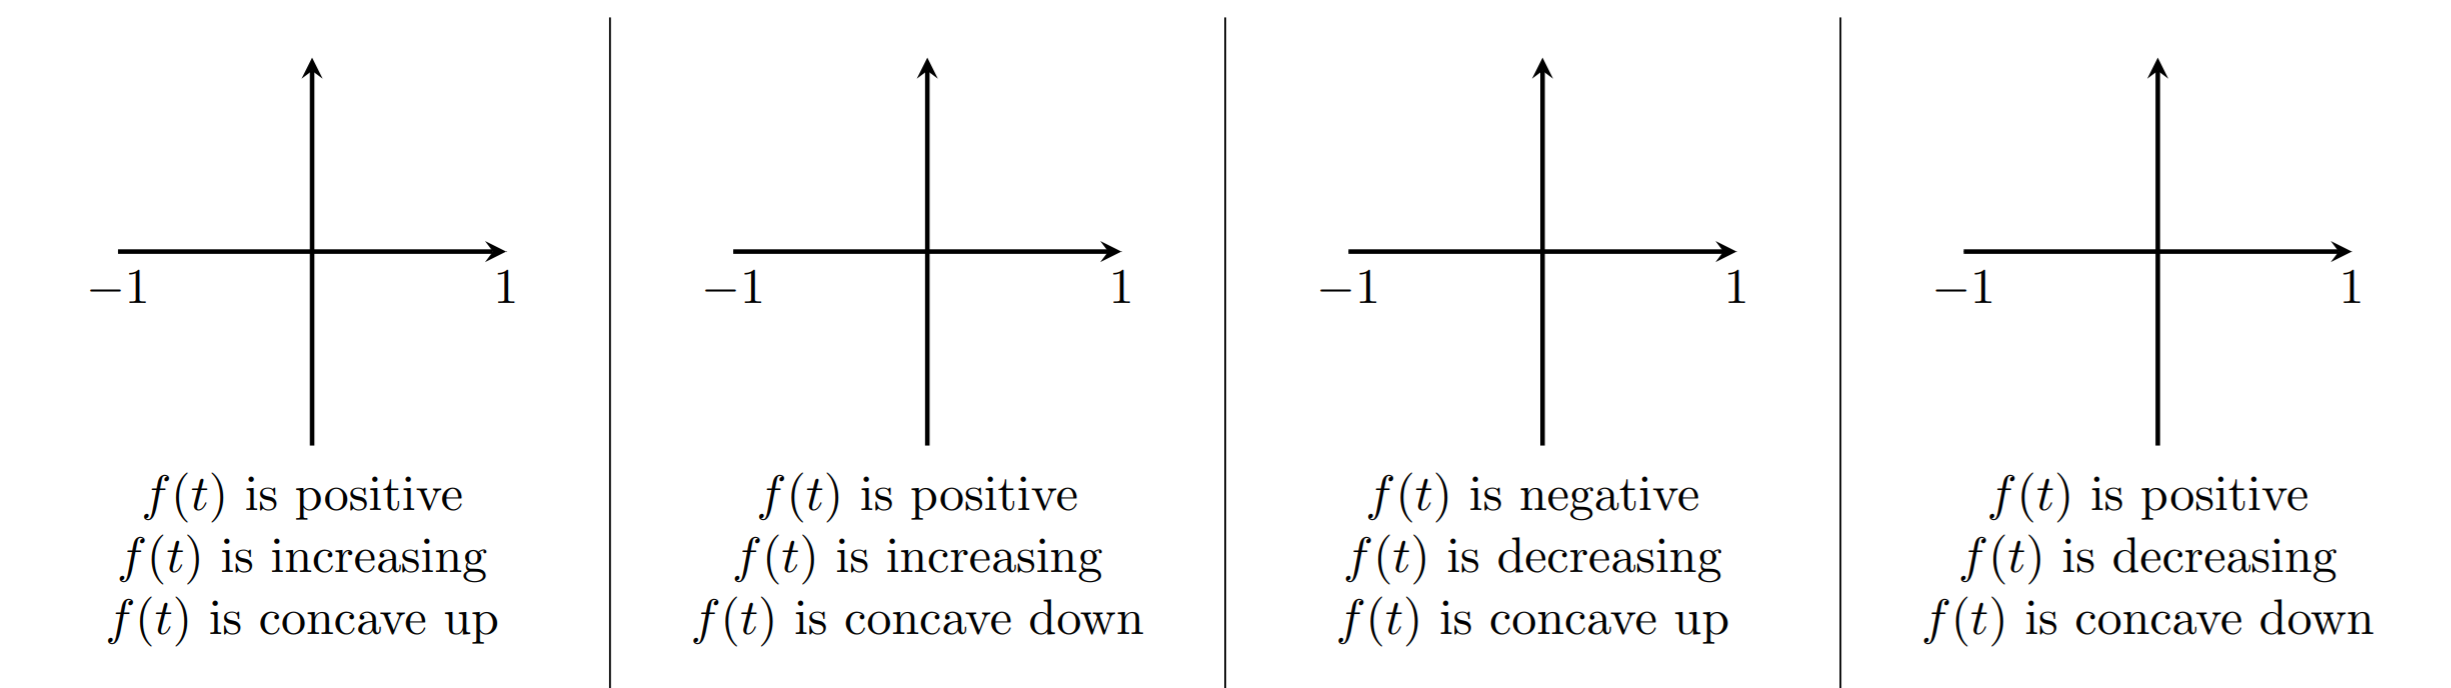
\includegraphics[width=\textwidth]{12-07P.png}
        \end{center}
\end{exercise}

\newpage
\section{Graph Sketching}

\begin{exercise}
        Consider the function $f(x) = 3x^4-8x^3 + 6x^2$.
        \begin{enumerate}[(a)]
        \item Find the critical points of $f$.
                \vfill
        \item Create a sign chart for the first derivative and determine the open intervals on which the function is increasing/decreasing.
                \vfill
        \item Find the local maxima and minima of $f$, if any exist. Find the local max/min values by plugging the $x$-values into the $f(x)$.
                \vfill
        \item Create a sign chart for the second derivative and determine the open intervals on which the function is concave up/down.
                \vfill
        \item Find any inflection points of $f$. Find the $y$-value at each inflection point by plugging the $x$-values into $f(x)$.
                \vfill
                \newpage
        \item Plot the local extrema and inflection points on the graph.
                Transfer the information from Parts (b) and (d) to the number lines for $f'(x)$ and $f''(x)$.
                Finally, sketch the graph of the function $f(x) = 3x^4-8x^3+6x^2$ using all of this information.
                \begin{center}
                        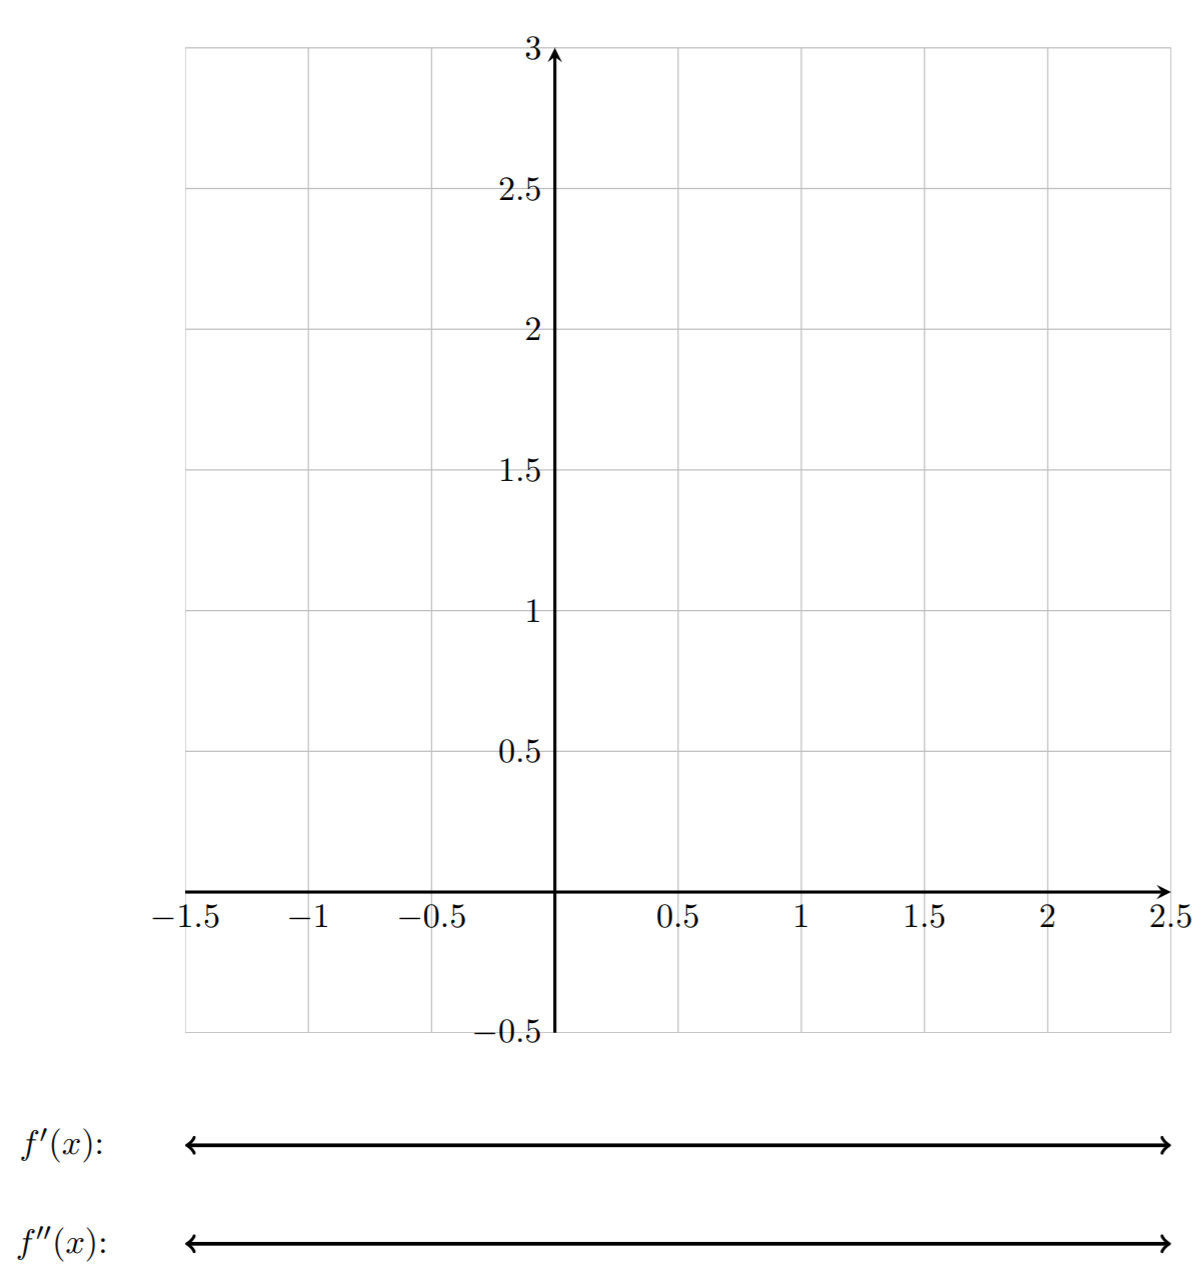
\includegraphics[width=.9\textwidth]{12-07P2.png} \qquad \qquad\qquad \qquad
                \end{center}
        \item Now use Desmos to get the graph of $y = f(x)$, and compare it to the graph you just drew. How well did you do?
        \end{enumerate}
\end{exercise}

\newpage

\begin{exercise}
        Using the same process as for Exercise 2, graph $f(x) = x^{1/3}(x+4)$ on the next page.
        \newpage
        \begin{center}
                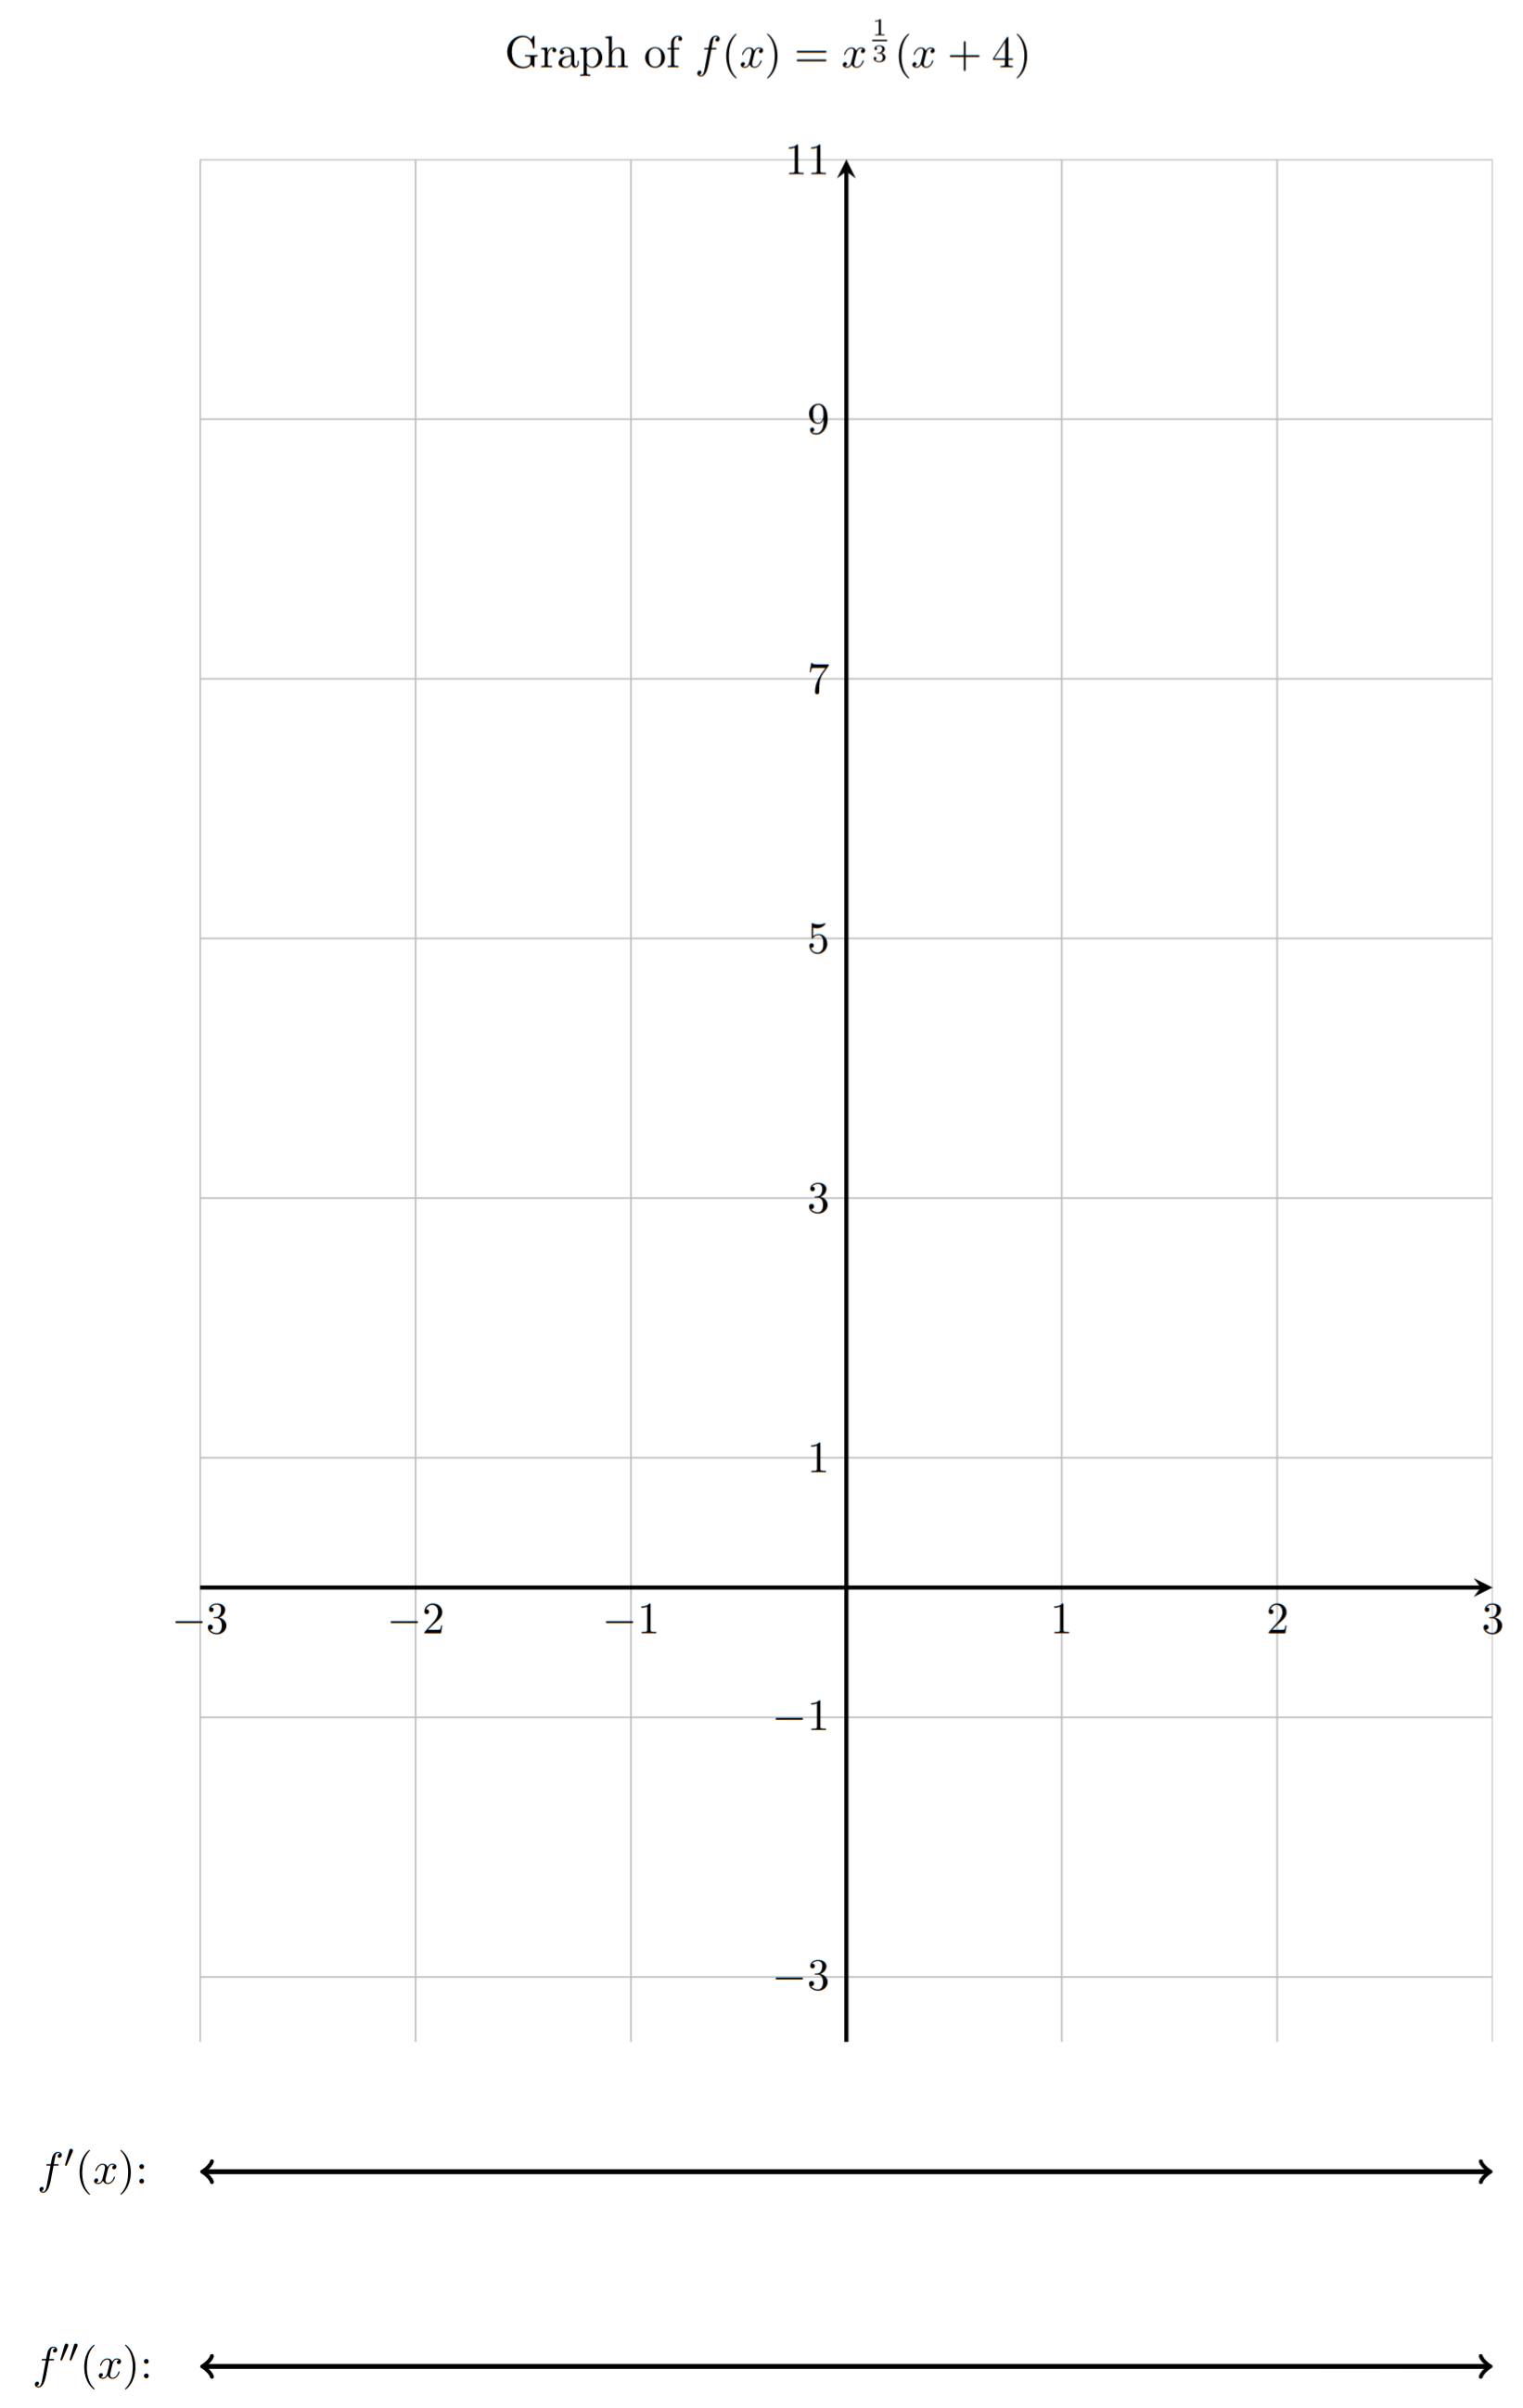
\includegraphics[width=.8\textwidth]{12-07P3.png} \qquad \qquad
        \end{center}
\end{exercise}
\end{document}
